\documentclass[conference]{IEEEtran}
\IEEEoverridecommandlockouts
% The preceding line is only needed to identify funding in the first footnote. If that is unneeded, please comment it out.
\usepackage{cite}
\usepackage{amsmath,amssymb,amsfonts}
%\usepackage{algorithmic}
\usepackage{graphicx}
\usepackage{caption}
\usepackage[utf8]{inputenc}
\usepackage[document]{ragged2e}
\usepackage[colorlinks=true, urlcolor=black, linkcolor=red]{hyperref}
\usepackage{textcomp}
\usepackage{xcolor}
\def\BibTeX{{\rm B\kern-.05em{\sc i\kern-.025em b}\kern-.08em
    T\kern-.1667em\lower.7ex\hbox{E}\kern-.125emX}}
\begin{document}
%\title{Report Title*\\
%{\footnotesize \textsuperscript{*}Note: Sub-titles are not captured in Xplore and
%should not be used}
%\thanks{Identify applicable funding agency here. If none, delete this.}
%}
\title{Impact of Video Games on Cognitive Abilities of Individuals}

\author{\IEEEauthorblockN{Student Name: Abhimanyu Negi}
\IEEEauthorblockA{Enrollment ID: \textbf{202001080} \\
B. Tech. Project (BTP) Report \\
BTP Mode: \textbf{\textit{On Campus} - in a Group*} \thanks{\textsuperscript{*}Group Members's Name: Preksha Anand,
 Enrollment ID: 202001061, Email: 202001061 [at] daiict.ac.in, Institute: DA-IICT} \\
\textit{Dhirubhai Ambani Institute of ICT (DA-IICT)}\\
Gandhinagar, India \\
202001080 [at] daiict.ac.in}
\and
\IEEEauthorblockN{Mentor's Name: Prof. Kalyan Sasidhar}
\IEEEauthorblockA{\textit{Dhirubhai Ambani Institute of ICT (DA-IICT)}\\
Near Indroda Circle \\
Gandhinagar 382007, India \\
kalyan\_sasidhar [at] daiict.ac.in}
%\and
%\IEEEauthorblockN{3\textsuperscript{rd} Given Name Surname}
%\IEEEauthorblockA{\textit{dept. name of organization (of Aff.)} \\
%\textit{name of organization (of Aff.)}\\
%City, Country \\
%email address}
}

\maketitle

\begin{abstract}
The gaming industry has seen a explosive growth in terms of revenue and active player base due to several technological advancements in console technologies which have made it accessible for everyone. This paper talks about how video games have a positive impact on cognitive abilities of individuals. It provides a detailed experimentation and statistical analysis in order to obtain the results. Lastly it discusses about the potentials of this experiment and also talks about the limitations which degrade the accuracy of these experiments.

\end{abstract}

\begin{IEEEkeywords}
Human Computer Interaction, Mental Chronometry, Reaction Time, Mouse Accuracy, Fitts Law, Hick-Hyman Law
\end{IEEEkeywords}

\section{Introduction}
The Gaming industry has gained a lot of momentum in recent years thanks to recent technological advancements, far reaching accessibility and acceptance of E Sports. This immense growth has propelled video games from mere niche hobby to a ubiquitous cultural force, permeating virtually every facet of modern society. 
\\
\begin{figure}[htp]
    \centering
    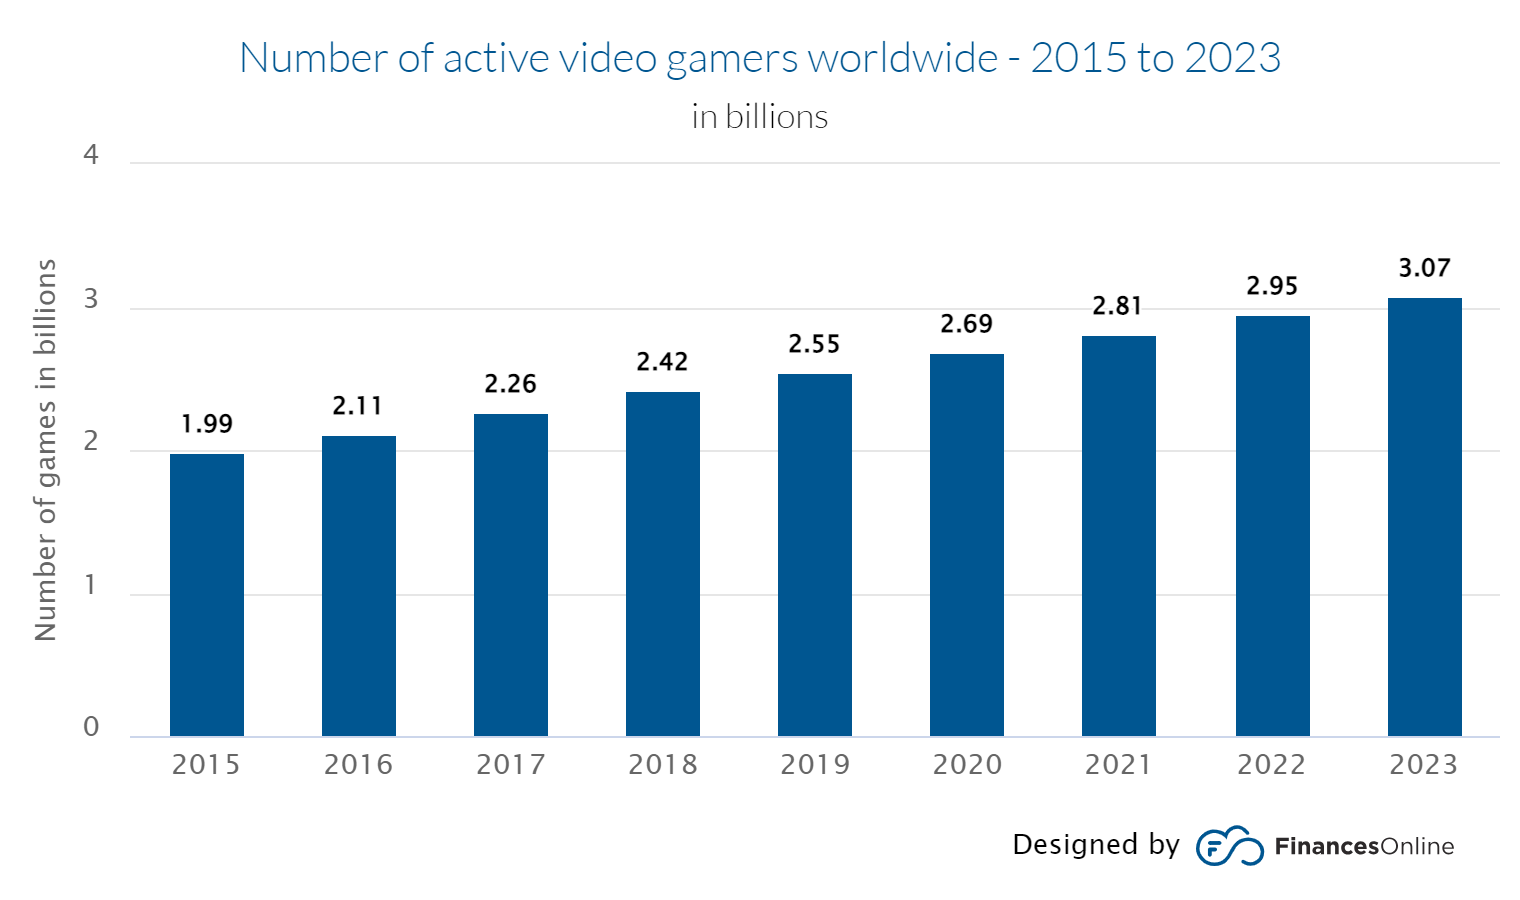
\includegraphics[width=9cm]{Number of Active Gamers.png}
    \caption{Number of Active Players [10]}
    \label{fig:Number of Active Players}
\end{figure}
Over the years, the gaming industry is seeing explosive growth in terms of active players as well as revues. The industry now has a valuation of around 282 billion USD with approximately 3.07 billion players across the Globe. This is due to the fact that Video games have come a long way, where it has now expanded from traditional PC and console gaming to modern portable handhelds and cloud gaming services. This expansion has transcended demographic boundaries and has captivated audiences of all ages.

\begin{figure}[htp]
    \centering
    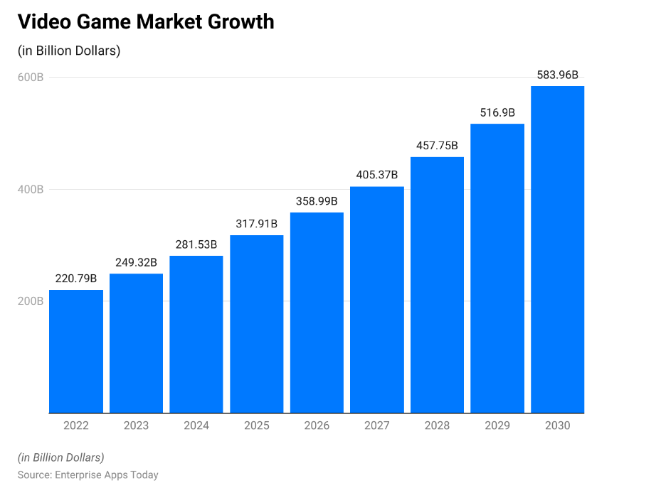
\includegraphics[width=9 cm,height=8.5cm]{revenue.png}
    \caption{Revenue of Gaming industry [9]}
    \label{fig:Revenue of Industry}
\end{figure}
\\
Along with the rise of the industry, there arises a question of “do video games actually have an impact on humans?”. In this paper we try to find a statistically correct answer to this question and find out if the impact is significant or not also if its positive or negative impact via means of different tests and experimentation followed by extensive statistical analysis.


\section{Learning Outcomes}
This research project helped us to understand and acquire different skills required to conduct such projects. Following is the list of the learning we had during the project.
\begin{itemize}
  \item Technical Skills
  \begin{enumerate}
      \item Research Methodology
      \item Data Collection and Analysis
      \item Experimental Design
      \item Statistical Analysis
      \item Data Visualization
  \end{enumerate}
  \item Non Technical Skills
  \begin{enumerate}
      \item Ethical Considerations
      \item Critical Thinking
      \item Problem solving
      \item Adaptability
      \item Collaboration Skills
      \item Time Management
  \end{enumerate}
\end{itemize}
\section{Contributions}
Following is the list of contributions

\subsection{My Individual Contribution}
\begin{itemize}
    \item Survey Analysis
    \item Handling Ethical Considerations
    \item Forming the Experimental Design
    \item Conducting and Observing the experiment for No Experience and Beginner Players
    \item Descriptive Statistics
\end{itemize}

\subsection{Other Members' Contributions}
\begin{itemize}
    \item Survey Analysis
    \item Explaining the Experimental Design to Participants
    \item Conducting and Observing the experiment for Amatuer and Professional Players
    \item Bland Altman Analysis and Box Plot Analysis
    \item Data visualisation
\end{itemize}
\section{Related Work}
\begin{flushleft}
    Video games have been under the radar of researchers for a very long time. Several questions have been put forward regarding the effects of videogames on different aspects of individuals whether be it psychological or mental capability etc. In order to answer some of these questions various researches have been performed.
\newline
In 2019, a research was conducted in order to find the association between videogames and its psychological factor [1]. The research focused on different factors like stress,distraction etc and assessed these values based on self assessment from the users using various standardized psychological assessment tests. The paper then covered various generalization scores in order to find the final scores for each of its participants and assess how the video games impacted each of their behavior. One of the problems which the paper highlighted that correlation might not explain the causation also the paper mentions how all of these tests which perform in such experimentation are mostly self-assessed and hence can have biases which may not provide accurate results and hence will differ from user to user. Such experimentation does not provide a general result and hence leaves the problem and its cause unexplained.
\end{flushleft}
\newline
\newline
\begin{flushleft}
    
Further research in the psychological field has always been inconclusive and does not apply to a general population due to different assessment methods and evaluation techniques. Research done in 2021 [3] gave justification for how video games impact well-being positively, while research done in 2022 [4] explains how video games do not impact well-being. Both researchers give their justification for their hypothesis and different statistics to prove the correctness of their hypothesis. Such inconclusive results are due to the use of self-assessment methods.
\end{flushleft}
\newline
\newline
\begin{flushleft}
    
In order to perform the experiment we chose a different aspect to the video games and looked at how video games can affect the cognitive abilities of individuals. We read various papers about Mental Chronometry [5] and its assessment methods. While going through literature review, we did not come across many papers which did an extensive experimentation on the same set of players. Hence we decided to do an experiment which could provide some answer to the question if video games affect cognitive abilities and if the effect is positive or negative.
\end{flushleft}
\newline
\newline
A paper about different evaluation methods using video games provided some hint about the genre of games which could be used for such an experiment [6]. After reading the paper we came to the conclusion that in order to perform the experiment we would need participants to play a shooter type game for over multiple sessions in order to get data for assessment of its impact on cognitive performance of the individuals.



\section{Study Methodology}
In order to understand how video games affect different individuals, the research experiment was conducted in 2 phases. 
\begin{enumerate}
    \item Phase One: Survey Analysis and 1 Week pilot experimentation
    \item Phase Two: 7 Week long experimental gaming sessions
\end{enumerate}
\subsection{Phase One}
The Phase One of the research was divided into the following two parts
\begin{enumerate}
    \item Survey and Background Analysis
    \item Pilot Experimentation
\end{enumerate}

\subsubsection{Survey and Background Analysis}
For the survey and background analysis a google form was circulated among the people of different ages in order to understand the different skill levels in the groups. Based on the different skill levels and past gaming experience, the participants were divided into 4 groups 
\begin{itemize}
    \item No Experience : 0 hours/week
    \item Beginner: 1-2 hours/ week
    \item Amateur: 3-4 hours/week
    \item Professional: 5+ hours/week
\end{itemize}

After collection of the data from the survey form, 30 participants from different age groups, gender and experience levels were selected for the pilot study and for participation in phase two of research.


\begin{figure}[htp]
    \centering
    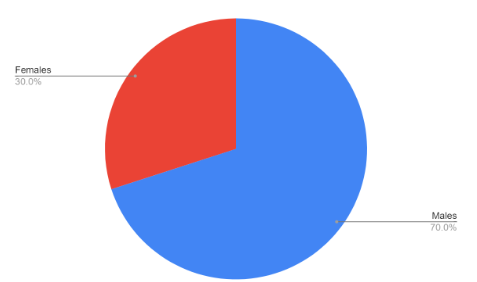
\includegraphics[width=5cm,height=3cm]{Gender distribution.png}
    \caption{Gender Distribution}
    \label{fig:Gender Distribution}
\end{figure}
\begin{figure}[htp]
    \centering
    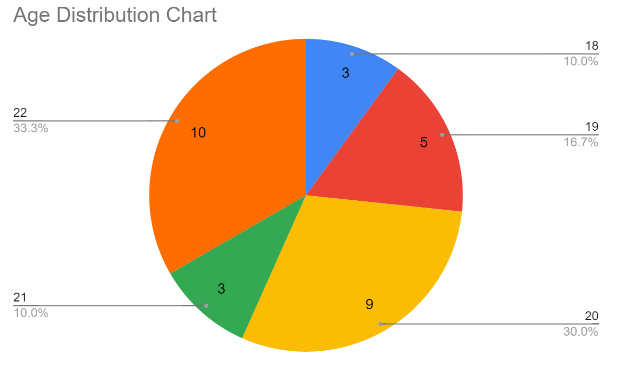
\includegraphics[width=7cm,height=4cm]{Age Distribution Chart.png}
    \caption{Age Distribution}
    \label{fig:Age Distribution}
\end{figure}
\begin{figure}[htp]
    \centering
    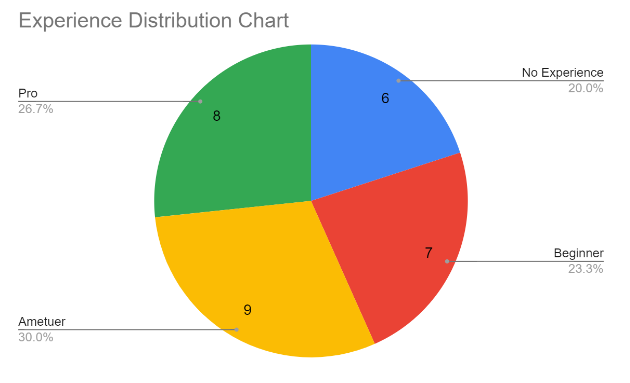
\includegraphics[width=7cm,height=4cm]{Experience Distribution.png}
    \caption{Experience Distribution}
    \label{fig:Experience Distribution}
\end{figure}

\subsubsection{Pilot Experiment}
For the Pilot experiment, we made each participant play games of different genres and did multiple cognitive tests in order to determine which possible genre with the combination of tests will help us in determining the impact of video games on the cognitive abilities. 
\\Each of the participants were observed for 1 week and several different tests were conducted and their experience of the tests were recorded and later analysed.
\\Based on the outcomes of this pilot experiment, the experimentation design of Phase Two was created.

\subsection{Phase Two}
Based on the experiment design from the results of Phase One a shooter game ie. Call of Duty 4: Modern Warfare was decided to be used as a part of the experiment. The experiment duration was set to 7 weeks.
\\
Each week participants would be expected to play the game twice (2 sessions) for 30 minutes/session. They were also asked to perform couple of tests before and after the session in order to analyze their cognitive behaviour.
\\
Two tests were selected to analyse the cognitive behaviour of the individuals and these are based upon the perceive-act cycle.

\begin{figure}[htp]
    \centering
    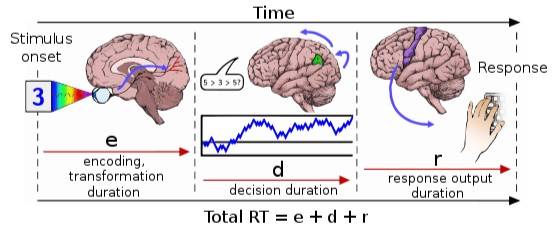
\includegraphics[width=9cm]{perceive-act cycle.png}
    \caption{Perceive-act cycle [11]}
    \label{fig:Perceive-act cycle}
\end{figure}

Figure 6 visualizes the perceive act cycle. It has the following 3 stages
\begin{enumerate}
    \item Encoding transformation duration: During this stage the eyes capture the stimuli and send information to the brain. \textbf{Range [50-200ms]}
    \item Decision duration: During this stage, the brain analyzes the stimuli and sends response to the respective motor organ.\textbf{Range [25-170ms]}
    \item Response output duration: During this stage, the response is received by the motor organ, and acts according to the stimuli.\textbf{Range [30-100ms]}
\end{enumerate}
\\
\centering \textbf{Reaction Time = Encoding Transformation Duration + Decision Duration + Response Output Duration}
\newline
\newline
\centering \textbf{RT($ms$) = e + d + r}
\newline
\newline
The following two tests were selected for the experiment
\begin{itemize}
    \item \textbf{\href{https://humanbenchmark.com/tests/reactiontime}{Reaction Time test}}: This test was selected in order to understand how much time does a participant take to react to a stimulus. 
    \begin{figure}[htp]
    \centering
    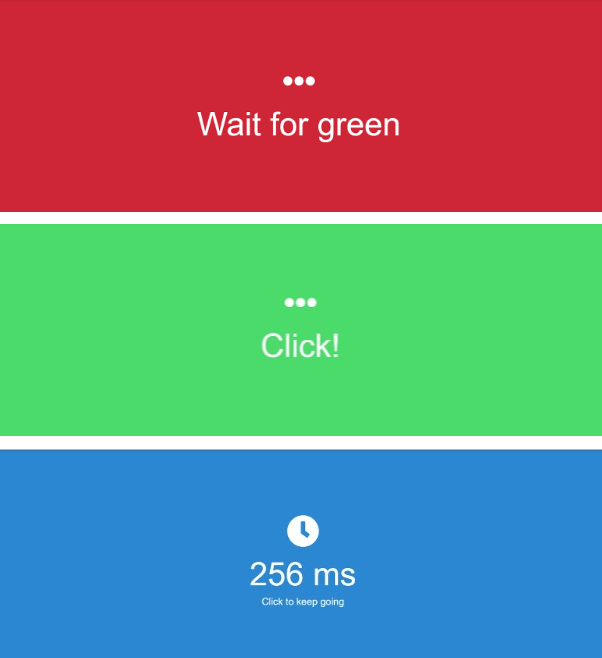
\includegraphics[width=6cm,height = 7cm]{RT combinied.png}
    \caption{Reaction Time Test [12]}
    \label{fig:Reaction Time test}
\end{figure}
\newline
\newline
    The test runs for four to five times and at the end an average of the test is given as the reaction time.
\newline
\newline

\item \textbf{\href{https://mouseaccuracy.com/}{Mouse Accuracy Test}}: This test was selected in order to understand how participants react to multiple targets on screen and try to hit each of them as they dynamically differ in sizes and vanish. This test is based on two important laws of Human Computer Interaction ie Fitt's Law and Hick Hymans Law.
\begin{figure}[htp]
    \centering
    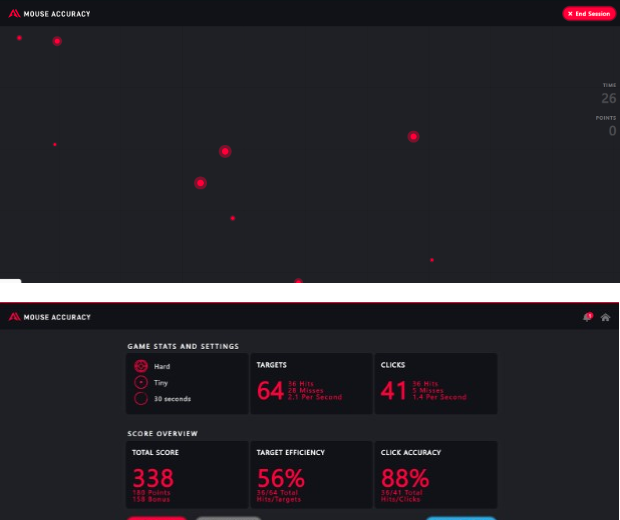
\includegraphics[width=8cm,height = 9cm]{MA combined.png}
    \caption{Mouse accuracy Test [13]}
    \label{fig:Mouse accuracy test}
\end{figure}
\newline
\newline
\newline
\textbf{Fitt's Law}: Fitts law predicts that the time required to rapidly reach a target is dependent on the distance (from the original location to the target location) and the size of the target. 
\newline
\newline
\textbf{Hick Hymans law}: Hick Hymans law is more on the psychological side and says that the decision time of a person increases as the number of choices given to that person increases.

\begin{figure}[htp]
    \centering
    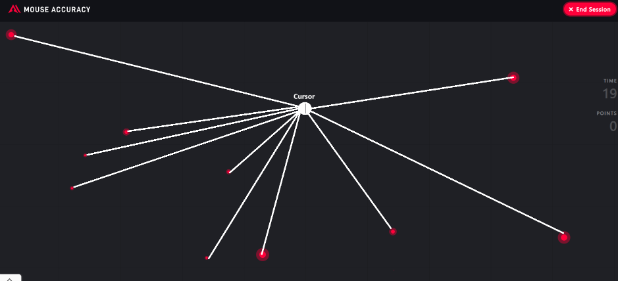
\includegraphics[width=8cm,height = 4cm]{Laws.png}
    \caption{Application of Fitts and Hick Hyman Law [13]}
    \label{fig:Application of Fitts and Hick Hyman Law}
\end{figure}

\end{itemize}

\newline
\newline
\RaggedRight As a part of the experimentation, the participants were asked to play the game twice a week and to perform the test before and after playing the game. This would go on for 7 weeks, with a gradual increase in the play time. This gave us data on how the user performed before and after the gaming session.
 
\newline\newline \newline

\RaggedRight Following the completion of 7 weeks. The data for each of the participant was compiled and further analyzed to obtain the results

\section{Research Findings}
\begin{flushleft}
    \subsection{Reaction Time Test}
    As the participants played the games for weeks, we can see a gradual decrease in the reaction time, though the change varies across the groups. The most improvement can be seen in the non-experienced players, then the beginner players, then the amateurs with minute changes, and the pro players with drops and rises in a particular range of reaction time.
\end{flushleft}
\newline
\newline
The non-experienced participants' initial mean after their first gaming session was 346 ms, which fell to 281 ms at the end of their experiment, with a standard deviation of approximately 35.5.
\newline
\begin{flushleft}
    For beginners, the average first gaming session time was 306 ms, which fell to 255 ms at the end of the last session. For amateur players, the first-week mean was 261 ms, which dropped to 224 ms. However, the mean of the pro players at the end of their first gaming session was 230 ms, which subsequently decreased to 214 ms, indicating a slight difference between the initial stage's reaction time and the final week's reaction time of the pro players.
\end{flushleft}

\begin{figure}[htp]
    \centering
    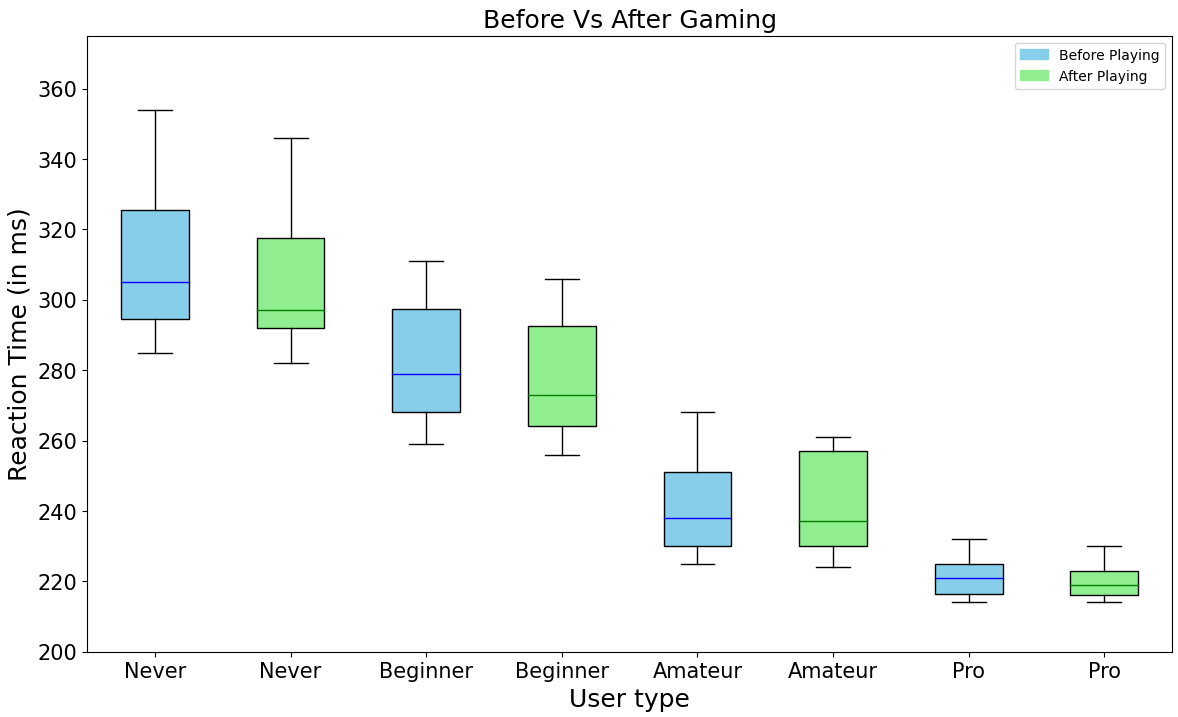
\includegraphics[width=9cm,height = 5.5cm]{Boxplot RC.png}
    \caption{Reaction Time Box plot analysis of groups of participants}
    \label{}
\end{figure}

\begin{figure*}[t]
\begin{center}
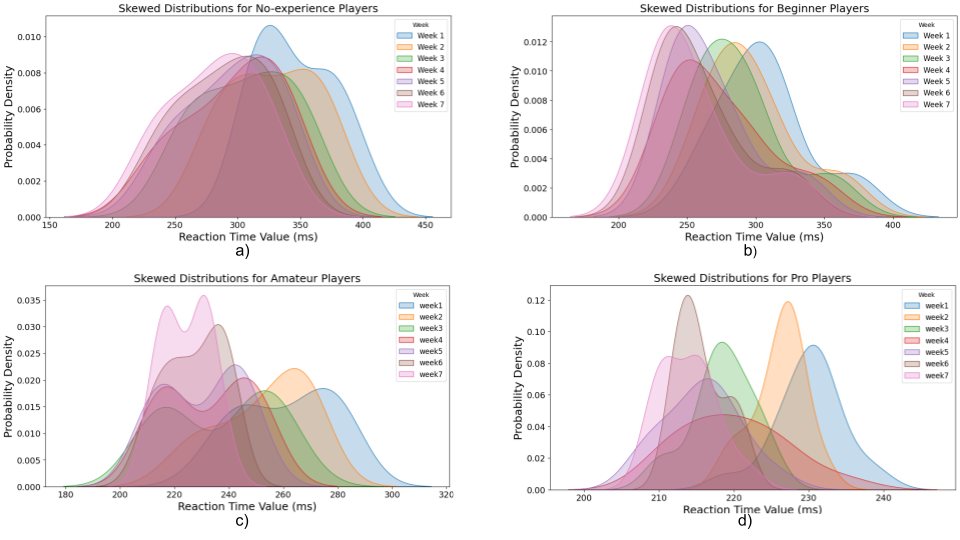
\includegraphics[width=18cm,height = 10cm]{SKD RC GROUP.png}
\end{center}
\caption{Skewed Distribution chart of Reaction Time}%
\label{label}
\end{figure*}

\begin{flushleft}
    The graph Fig.10 shows the reaction times of each group before and after playing video games. We can see that the median of each group is reduced after playing video games. 
\end{flushleft}



 
\begin{flushleft}
We can also infer some similarity between non-experienced and beginner players, as well as a significant difference between non-experienced and professional players' behaviors.
\end{flushleft}
\newline
\newline
\begin{flushleft}

    From the skewed distribution (Fig 11 a,b,c,d) we can say that the group of non-experienced and amateur players gives a negatively skewed distribution (i.e., mean $<$ median $<$ mode), whereas the group of beginners and professional players gives a positively skewed distribution (i.e., mode $<$ median $<$ mean).
    \newline
    Also, in each group, the skewed curve is shifting towards the origin, indicating a decrease in the reaction times per week. There is a steady shift for the group of inexperienced, beginners and amateur players, while there is a inconsistency in the professional player’s shift. 
    \newline
When we observe the closing, we notice that there are skewed curves with more than one peak; that is, they are bimodal distributions, implying that the distribution has two modes.
\end{flushleft}
\subsection{Mouse Accuracy}
\begin{flushleft}
    

As the participants were instructed to play a first-person shooter game it helped them accelerate their mouse movements.
After every gaming session, the participants had increased their mouse accuracy score (no units). The most significant rise is seen in the non-experienced players. The group's initial average was 170, which became 222.
\end{flushleft}


\newline
\begin{figure}[htp]
    \centering
    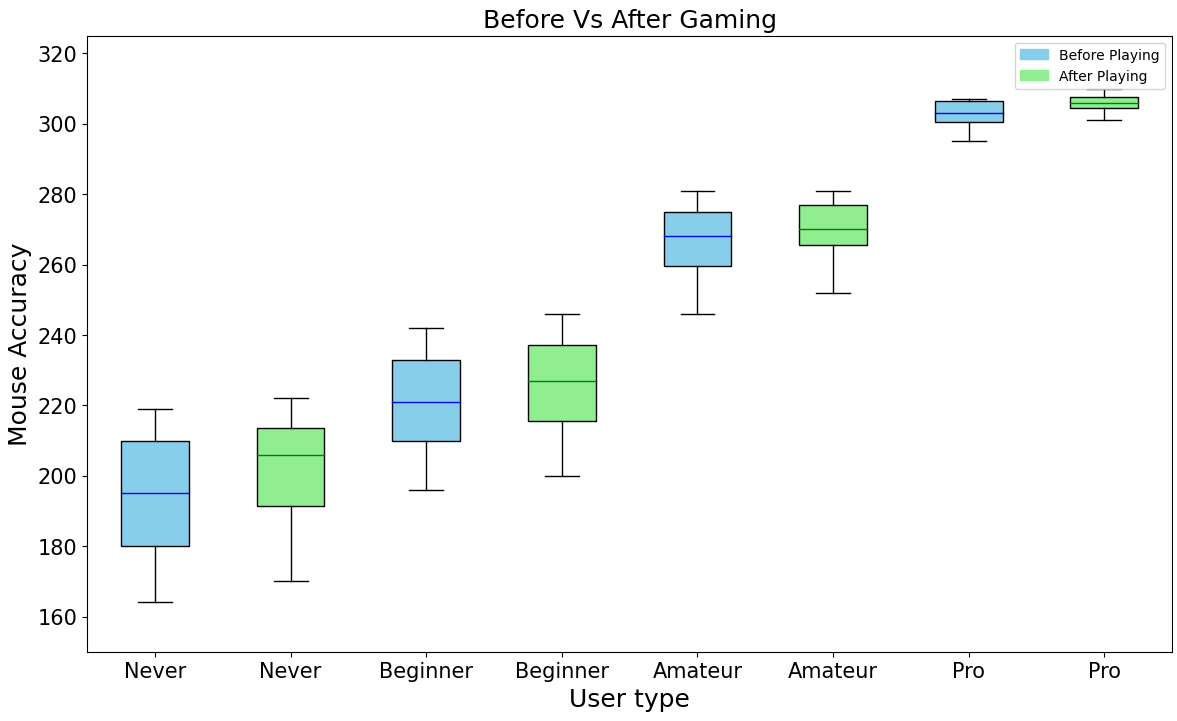
\includegraphics[width=9cm,height = 5.5cm]{Boxplot MA.png}
    \caption{Mouse Accuracy Box plot analysis of groups of participants}
    \label{}
\end{figure}
\begin{flushleft}
The box plot (Fig 12) shows us the change in the mouse accuracy score before and after playing video games. This plot takes up the data collected over the seven-week period.
\end{flushleft}

\begin{flushleft}
We can see a rise in the median in all the groups, with some showing a significant increase while others have a minor increment. The beginners had an average of 200 in\end{flushleft}



\begin{figure*}[t]
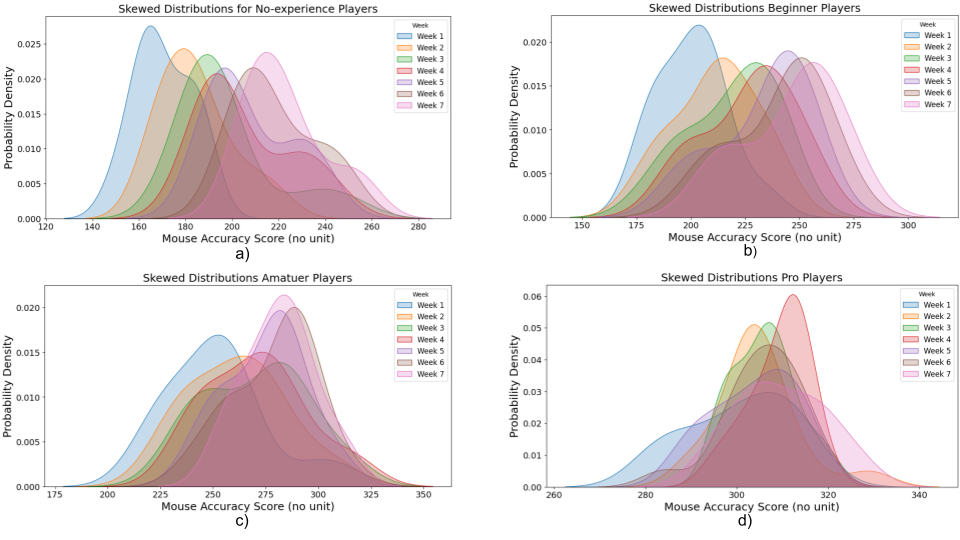
\includegraphics[width=18cm,height = 10cm]{SKD MA GROUP.png}
\caption{Skewed Distribution chart of Mouse Accuracy}%
\label{label}
\end{figure*}

\begin{flushleft}
the first week and 246 in the last week. In the amateurs, we can see a change from 252 to 280. While in the professional players, the initial mean was 300, which had a negligible increase to 309 even overall range of the professionals remains the same.
\end{flushleft}

\begin{flushleft}
    The skewed distribution plots (Fig 13 a,b,c,d) show us that the non-experienced players have a positively skewed distribution, while the beginners have a negatively skewed distribution. The amateurs and the professional players show ambiguous results across the seven weeks. Although the skewed curves show a shift away from the origin, indicating an increase in mouse accuracy score, there is essentially almost no shift in the professional player group.
\end{flushleft}


\subsection{Correlations between the groups}

\begin{flushleft}
    A few patterns can be identified among the four groups based on the collected data. The non-experienced and the beginners behave similarly, as do amateurs and professionals. The main variation in trends can be noted between the non-experienced and the professionals. The inexperienced improved significantly in both tests, whereas professionals reached a point where they fluctuated in both tests.


\end{flushleft}

\begin{figure}[htp]
    \centering
    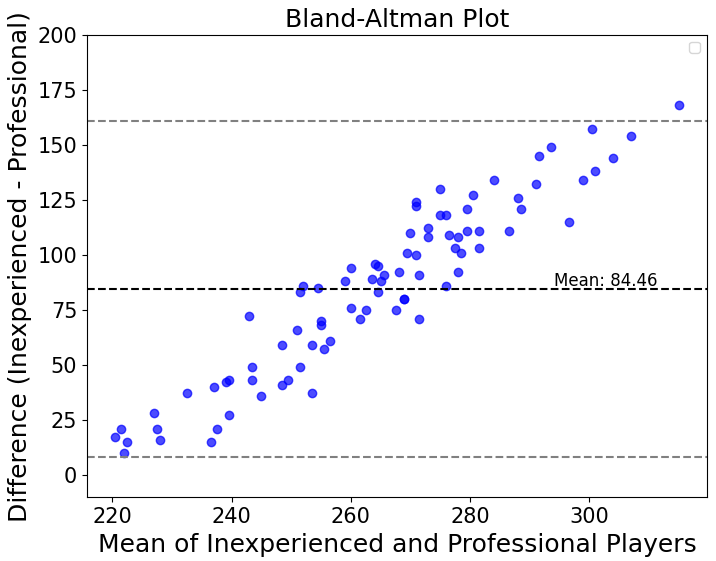
\includegraphics[width=8cm,height = 6.5cm]{BlandAltman Never n Pro.png
    }
    \caption{Bland Altman Analysis plot between in-experienced and Professional players}
    \label{}
\end{figure}
\begin{flushleft}
    The dispersed points in the plot in figure 14 between the inexperienced and the professional indicate that the groups produce a wide range of outputs and do not follow a similar trend. The mean difference between these is 84.46, which is extremely large.
\end{flushleft}
\begin{figure}[htp]
    \centering
    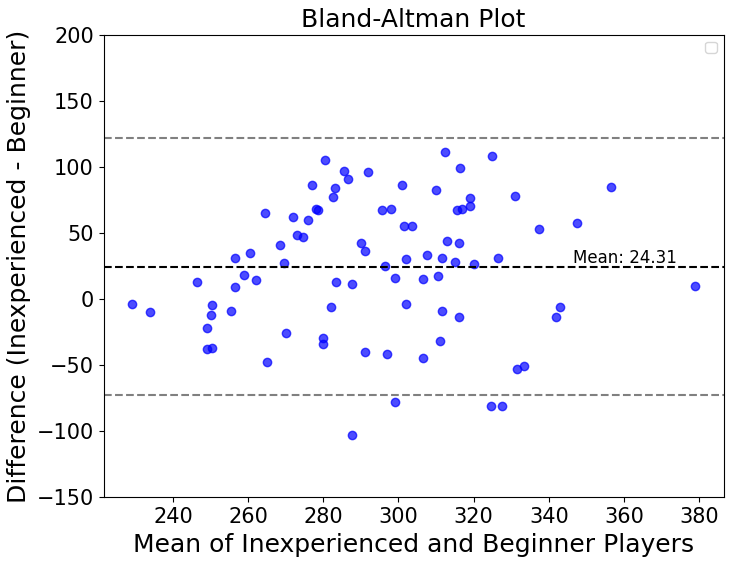
\includegraphics[width=8cm,height = 6.5cm]{BlandAltman Never n Beginner.png}
    }
    \caption{Bland Altman Analysis Plot between in-experienced and Beginner Players}
    \label{}
\end{figure}
\begin{figure}[htp]
    \centering
    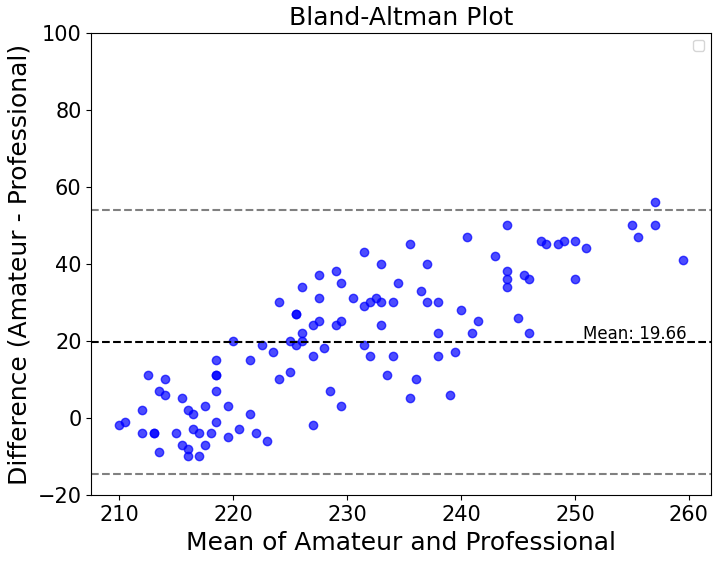
\includegraphics[width=8cm,height = 6.5cm]{BlandAltman AmateurnPro.png}
    }
    \caption{Bland Altman Analysis Plot between Amateur and Professional Players}
    \label{}
\end{figure}
\begin{flushleft}
    The points in plots figure 15 and figure 16 are not evenly distributed across the graph and are closely grouped together, implying that amateurs, professionals, and inexperienced, beginner players behave similarly. The mean difference between amateurs and pros is 19.66, which is even lower than 24.31 for inexperienced and beginners, indicating that their trends are more similar.
\end{flushleft}

\section{Discussion}
\begin{flushleft}
    The main question that we focused on throughout the research was how video games are affecting the cognitive abilities of individuals. The experiments helped us to find if the effect of video games is significant enough and whether it is positive or negative.
\end{flushleft}
\newline
\newline
\begin{flushleft}
    However, this experiment is just a small part of the research that can be done in this particular field. Perspectives from the field of Psychology and Human behavior will help in understanding the effects of video games on the overall personality of the individual apart from just cognitive behavior.  
\end{flushleft}
\newline \newline
\begin{flushleft}
    Our experiment has a few limitations like a small population set which only had a few participants from very similar ages. Apart from that the small duration of the experiment as well as just 2 sessions per week gives us less data to work with and get more precise results.
\end{flushleft}

\begin{flushleft}
    Getting a large number of participants from varying ages and experience levels will enable us to get a more general idea about the impact of video games and help gather more useful information to statistically analyze. The frequency of sessions per week combined with a longer run of the experiment will help us to gather more data from the participants which can then be used to perform linear regression and different analysis models. 
\end{flushleft}
\section{Conclusion}
\begin{flushleft}
Modern day gaming industry has evolved from what it was back just 10-15 years ago. Thanks to thousands of gaming titles spanning across different genres, video games have evolved from a niche hobby to a ubiquitous culture. This explosive growth has led to several researches on how these video games affect individuals. 

Throughout this paper, we did several analyses of the data we collected from the 30 participants throughout the duration of the experiment. From the analysis, we realized that all the participants had a positive impact on their cognitive skills, though there were few participants who had tremendous improvement while others had a slight growth. Video gaming had a greater positive impact on the users who never or rarely play, that is, the inexperienced and the beginner participant groups. The other groups of participants, amateur and professional players, remained in a particular range but kept fluctuating in the test results. 
    
\end{flushleft}

\begin{thebibliography}{00}
\bibitem{b1}Juliane M. von der Heiden,Beate Braun,Kai W. Müller,Boris Egloff [2019], "The Association Between Video Gaming and Psychological Functioning",\href{https://doi.org/10.3389/fpsyg.2019.01731}{https://doi.org/10.3389/fpsyg.2019.01731}
\bibitem{b2} Chaarani B, Ortigara J, Yuan D, Loso H, Potter A, Garavan HP. Association of Video Gaming With Cognitive Performance Among Children [2022]. JAMA Netw Open. 2022;5(10):e2235721. \href{doi:10.1001/jamanetworkopen.2022.35721}{doi:10.1001/jamanetworkopen.2022.35721}
\bibitem{b3}Niklas Johannes†, Matti Vuorre† and Andrew K. Przybylski[2021], "Video game play is positively correlated with well-being", \href{https://doi.org/10.1098/rsos.202049}{https://doi.org/10.1098/rsos.202049}
\bibitem{b4} Matti Vuorre†, Niklas Johannes†, Kristoffer Magnusson and Andrew K. Przybylski [2022],"Time spent playing video games is unlikely to impact well-being"\href{https://doi.org/10.1098/rsos.220411}{https://doi.org/10.1098/rsos.220411}
\bibitem{b5} Kranzler, J.H. (2012). Mental Chronometry. In: Seel, N.M. (eds) Encyclopedia of the Sciences of Learning. Springer, Boston, MA. \href{https://doi.org/10.1007/978-1-4419-1428-6_238}{https://doi.org/10.1007/978-1-4419-1428-6_238}
\bibitem{b6}Jayne Gackenbach,Matt Rosie (2009) "Cognitive evaluation of video games: players' perceptions" \href{https://doi.org/10.1145/1639601.1639615}{https://doi.org/10.1145/1639601.1639615}
\bibitem{b7}C. Shawn Green, Aaron R. Seitz (2015), "The Impacts of Video Games on Cognition (and How the Government Can Guide the Industry)" \href{https://doi.org/10.1177/2372732215601121}{https://doi.org/10.1177/2372732215601121}
\bibitem{b8} Giavarina, Davide. (2015). Understanding Bland Altman analysis. Biochemia Medica. 25. 141-151. 10.11613/BM.2015.015.
\bibitem{b9} Barry Elad, "Video Game Industry Statistics 2024" \href{https://www.enterpriseappstoday.com/stats/video-game-industry-statistics.html}{https://www.enterpriseappstoday.com/stats/video-game-industry-statistics.html}
\bibitem{b10}Nestor Gilbert, "Number of Gamers Worldwide 2024", \href{https://financesonline.com/number-of-gamers-worldwide}{https://financesonline.com/number-of-gamers-worldwide} 
\bibitem{b11}Wikipedia: \href{https://en.wikipedia.org/wiki/Mental_chronometry#Standard_reaction_time_paradigms}{https://en.wikipedia.org/wiki/Mental_chronometry}
\bibitem{b12}Human Benchmark:
\href{https://humanbenchmark.com/tests/reactiontime}{https://humanbenchmark.com/tests/reactiontime}

\bibitem{b13}Mouse Accuracy: \href{https://mouseaccuracy.com/}{https://mouseaccuracy.com/}

\bibitem{b14} Donovan I, Saul MA, DeSimone K, Listman JB, Mackey WE and Heeger DJ (2022) Assessment of human expertise and movement kinematics in first-person shooter games. Front. Hum. Neurosci. 16:979293. doi: 10.3389/fnhum.2022.979293


\end{thebibliography}

\end{document}
